\documentclass[letterpaper]{article}

\usepackage[english]{babel}
\usepackage[utf8]{inputenc}
\usepackage{graphicx}
\usepackage{listings}
\usepackage[superscript,biblabel]{cite}

\title{Blocky: A Generalized Blockchain-Oriented Programming Language}

\author{Matthew Leeds (mwleeds@crimson.ua.edu)}

\date{November 23, 2015}

\begin{document}
\maketitle

\begin{abstract}
Ever since 2009 when Satoshi Nakamoto released the first workable blockchain-based application, Bitcoin, the technology has been an area of much interest, research, and development both in academia and the private sector. While Bitcoin uses cryptographically linked ``blocks" of transactions to transfer money over the Internet, the decentralized consensus technology can be applied to a wide range of problems from censorship-resistant content hosting to autonomous corporations to self-enforcing smart contracts. However there does not exist a common framework for the development of such apps with minimal effort on the developer's part and defined interoperability between them. Blocky seeks to fill this hole by providing a language for the creation of arbitrary blockchain-based applications.
\end{abstract}

\section{Introduction}

Bitcoin, Namecoin, Storj, and many other projects utilize very similar underlying cryptographic blockchains, each with unique application logic to serve the desired purpose (transfer money, register domain names, store files, etc). Because they each have separate blockchains, they each must convince users to run nodes in order to make the networks useful, and they must maintain a sizable code base to handle processing and propagation of blocks. If they could all be written in a well-defined common language, they could run on any compatible blockchain and thus would be much easier to develop and maintain.

The Ethereum project seeks to provide a blockchain, cryptocurrency, and language for deploying arbitrary blockchain apps, but its language (Solidity) only works in that system, whereas Blocky programs could be used on a variety of blockchains (whose cryptographic ciphers and transaction validation rules may differ) without changing their code. This can be accomplished because Blocky defines a set of interfaces that valid programs must implement as well as restrictions on usable language features to ensure well-behaved programs that can serve a wide range of potential purposes. Differences between Blocky and Solidity will be discussed further in a later section.

\section{The Blockchain Concept}
As implemented in the Bitcoin project, a blockchain is an append-only list of transactions in which later records are cryptographically linked to earlier ones in order to make modifying history computationally unfeasible. A symmetric key scheme is used to prove ownership over finite resources (such as bitcoins). Specifically, a user signs enough information to determine the origin and destination of the resource to be transferred using their private key.

\begin{figure}[h]
\centering
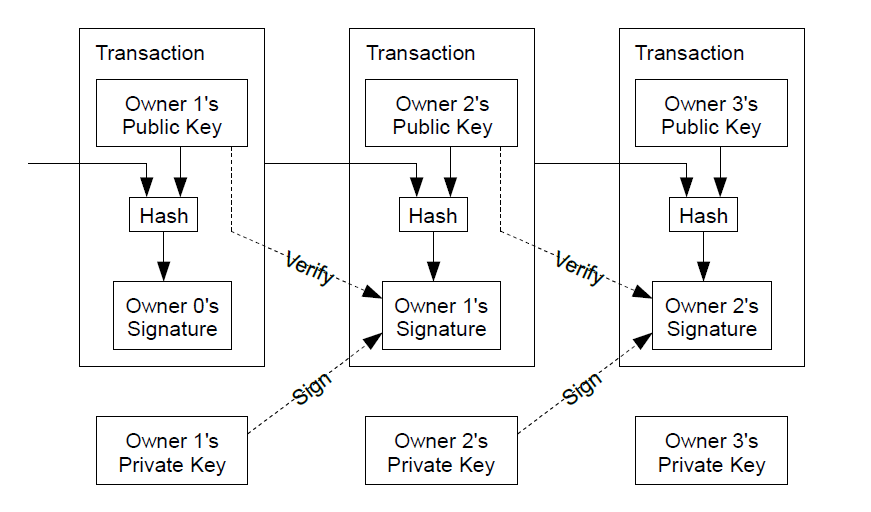
\includegraphics[width=0.7\textwidth]{transaction_chain.png}
\caption{\label{fig:transaction_chain}This is a simplified representation of transaction verification\cite{nakamoto09}.}
\end{figure}

This concept of transactions is generalized in Blocky so they can be used not just to transfer ``coins" but to send messages to dapps that trigger operations.

In addition to verifying individual transactions, cryptography must again be used to arrive at decentralized consensus as to which transactions are considered valid and have been executed. The primary mechanism for this is including the hash of the previous block when determining the hash of each block. This way, modifying the historical record of transactions without changing the hash values requires either knowledge of a major vulnerability in the algorithm that's used or a prohibitive amount of computing power (for brute forcing).

\begin{figure}[h]
\centering
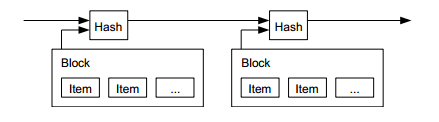
\includegraphics[width=0.7\textwidth]{blockchain.png}
\caption{\label{fig:blockchain}This is a high-level view of a blockchain\cite{nakamoto09}.}
\end{figure}

\section{Blocky's Execution Environment}

Blocky programs can execute on any computer running the software with a copy of the current blockchain. The host makes certain variables available to them, such as the current time and information about blockchain transactions. When a transaction occurs that has a message for a certain program, that program's \texttt{transact} method is called which validates the input and determines an appropriate course of action using its defined functions. The only ``side-effects" programs can have outside of their own stack variables is by broadcasting their own transactions to the network.

\section{Desirable Language Qualities}

The constraints and requirements of a blockchain ecosystem roughly dictate the following qualities that would maximize the usefulness of Blocky:
\begin{itemize}
  \item{Guaranteed termination or restricted computation time}
  \item{Turing completeness or as close as possible}
  \item{Access to relevant blockchain information}
  \item{No access to other resources on the host computer}
  \item{Definition of a standard interface for communication between apps}
  \item{Familiarity for users of existing languages}
  \item{A library of useful modules}
  \item{A balance between efficiency and ease-of-use}
\end{itemize}

The first and second points represent an unavoidable trade-off between arbitrary computation (Turing completeness) and guaranteed termination. Restricted computation time is important so that users cannot craft malicious or naive code that uses the computational resources of the host computer for an indefinite period of time. Unfortunately the only way to guarantee termination is to make the language less than Turing complete, meaning it will be possible to implement certain classes of algorithms\cite{turing37}. Limiting the language's expressiveness also means the code can be more easily understood, both by humans and computers\cite{plant15}.

The third and fourth points regarding access to information are primarily security concerns. If peers could run truly arbitrary code on each other's computers, this would very quickly lead to OS vulnerabilities being exploited and clients could easily be compromised by malicious actors. But data access cannot be restricted entirely because programs must at least be able to send and receive information relevant to their activities in order for the system to be useful. By specifying well-defined interfaces for such messages, Blocky solves this problem.

If an interface for communication between program instances is defined by the language rather than individual projects, it will be more universal and therefore reduce unnecessary compatibility issues.

To reduce the learning curve and speed adoption, the language should feel familiar to users of popular languages, at least in its basic syntax, and ideally in its semantics to the extent possible. Compiling to an existing language accomplishes this aim as many people already have some knowledge of how to use it.

To maximize usefulness the language should have a set of available modules comparable to the ones available for Python, Perl, and many others that support common tasks such as evaluation of non-trivial mathematical functions and parsing of regular expressions. By compiling to an existing language, we can avoid having to rewrite this technical infrastructure.

As mentioned above, efficient computation is an important consideration and much could be learned from C-style languages in this regard. But ease-of-use is arguably equally important because it makes developers more productive, as idealized by Python. Blocky seeks to arrive at a reasonable balance between these two extremes.

\section{Language Design and Specification}

Blocky is designed to share a significant amount of syntax and semantics with C\texttt{++}. Apart from providing familiarity, this makes it well-suited for efficient numerical computations, which are likely to be common (for example, cryptographic operations will occur frequently).

Similar to how classes are defined, \texttt{dapps} (decentralized applications) can be defined which have a single public method, \texttt{transact}, and any number of private methods. Here is the general layout of such a program:
\begin{lstlisting}
dapp MyDapp {
  public:
    transact(fixed_size_message); // the primary entry point
  private:
    // possibly other helper functions
}
\end{lstlisting}

They can also have state which is represented by a key value store, but changes to that must occur through transactions.

\subsection{Data Types}
Variables in Blocky are statically typed--- their types must be declared before they can be used. This system makes the code more explicit and readable, and protects against implicit variable declarations that may be accidental. Unlike C, Blocky uses strong typing so variables cannot be cast to other types and must be treated as their declared types. This can catch errors at compile-time in which the wrong variable is used in a statement. Further, numeric data types must explicitly declare their size in bytes (i.e. \texttt{int32\_t} or \texttt{int256\_t}, not just \texttt{int}). This rule makes potential for arithmetic overflow more obvious and forces code to execute comparably on different architectures (at least in this regard).

Static typing, strong typing, and explicit numeric types all lead to code that is more reliable, maintainable, and portable. 

\subsection{Scopes}
Scopes of variables available to Blocky programs:
\begin{itemize}
  \item{variables in their own stack and key-value store}
  \item{variables defined by the host, such as the current time}
  \item{blockchain-level variables which include information about transactions}
\end{itemize}
As with C\texttt{++}, \texttt{this} is used to access class (dapp) variables. Analogously, \texttt{host} and \texttt{chain} are used to access variables in the other scopes mentioned.
\newline

\subsection{Major Restrictions Relative to C\texttt{++}}
\begin{itemize}
  \item{\texttt{while} loops are not permitted}
  \item{\texttt{for} loops must have a deterministic invariant that will lead to termination}
  \item{\texttt{GOTO} statements and \texttt{switch} statements are not permitted}
  \item{Code is not permitted to access anything outside its own data and that of the blockchain (filesystem, network, etc)}
  \item{Code must implement the \texttt{transact} method}
  \item{strong typing}
  \item{Function arguments can differ at run-time}
\end{itemize}

\subsection{Compilation}
Steps taken by the Blocky compiler:
\begin{enumerate}
  \item{Remove comments and whitespace}
  \item{Validate the syntax of the code (check brackets, semicolons, etc)}
  \item{Ensure that no side-effects are allowed outside of the dapp and blockchain}
  \item{Ensure all data types are properly bounded (i.e. 32 bit integers)}
  \item{Do termination analysis to guarantee finite computation time (check \texttt{for} loop invariants, etc)}
  \item{Dynamically link the code based on the blockchain addresses of dapps that are transacted with}
\end{enumerate}

\section{Examples}

Some examples of decentralized apps that could be built using Blocky:
\begin{itemize}
  \item{A minimal-overhead, market-based cryptocurrency exchange}
  \item{A trustless exchange system for real-world goods and services (assuming there exists a reliable out-of-band way to verify receipt of such goods)}
  \item{A trustless crowdfunding platform}
  \item{A censorship-resistant content hosting platform}
\end{itemize}

\section{Comparison to Solidity}

Primary differences:
\begin{itemize}
  \item{Solidity code requires a virtual machine\cite{ethereum15}; Blocky code does not.}
  \item{Ethereum Virtual Machine instructions are restricted to 256-bit word operations\cite{ethereum15}.}
  \item{Addresses in Solidity are restricted to 160 bits\cite{ethereum15}.}
  \item{Solidity contracts must use Ether\cite{ethereum15}.}
\end{itemize}

\section{Potential Improvements}
To afford scalability, a mechanism could be provided so programs would only need to be executed on a subset of participating nodes, rather than the entire network. Similarly, a mechanism for parallelizing code would help Blocky make more efficient use of available resources.

\begin{thebibliography}{9}

\bibitem{nakamoto09}
  Satoshi Nakamoto,
  ``Bitcoin: A Peer-to-Peer Electronic Cash System",
  http://bitcoin.org/bitcoin.pdf
  
\bibitem{turing37}
  Alan Turing,
  ``On Computable Numbers, With an Application to the Entscheidungs Problem",
  Proc. London Math. Soc. (1937) s2-42 (1): 230-265.
  doi: 10.1112/plms/s2-42.1.230.
  
\bibitem{plant15}
  Luke Plant,
  ``We Need Less Powerful Languages",
  Published 14 November 2015.
  http://lukeplant.me.uk/blog/posts/less-powerful-languages/.
  
\bibitem{ethereum15}
  Solidity Documentation
  https://ethereum.github.io/solidity/docs/home/

\end{thebibliography}
  
\end{document}
